\documentclass[journal]{IEEEtran}

\usepackage[utf8]{inputenc}
\usepackage[T1]{fontenc}
\usepackage{amsmath,amssymb}
\usepackage{textcomp}
\usepackage{graphicx}
\usepackage{booktabs}
\usepackage{array}
\usepackage{url}
\usepackage{xcolor}

\graphicspath{{../figures/}}

\begin{document}

\title{Wire-Level Latency of On-Sensor MLC versus Host Inference on a Resource-Constrained Edge Platform: A Pre-Registered Measurement Study}

\author{Akul~Swami%
\thanks{Manuscript submitted \today.}%
\thanks{A.~Swami is an independent researcher (e-mail: swami.akul@alumni.uml.edu).}%
\thanks{Code, data, and the full pre-registration chain are available at https://github.com/akulswami/sensor-mlc-latency.}}

\markboth{IEEE Sensors Letters}{Swami: Wire-Level Latency of On-Sensor MLC versus Host Inference}

\maketitle

\begin{abstract}
The Machine Learning Core (MLC) embedded in the STMicroelectronics LSM6DSOX IMU is widely cited as a low-latency alternative to host-side inference, yet end-to-end wire-level latency is rarely measured. Using a Saleae Logic Pro 8 logic analyzer on an NVIDIA Jetson Orin Nano, we measured interrupt-to-decision latency (sensor INT1 edge to host decision GPIO) for three pipelines (a host-side decision-tree classifier, the standard MLC bank-switch read protocol, and an MLC binary-fast variant) under idle, I\textsuperscript{2}C bus contention, and CPU stress. The protocol was pre-registered with 12 externally-timestamped Zenodo amendments before confirmatory data collection (4,770 of 4,860 trials included, 98.15\%, across nine cells). The host pipeline exhibits lower median latency than the MLC pipeline under all conditions: 321.7 vs 681.5 $\mu$s at idle (2.1$\times$ faster) and 574.5 vs 1,325.4 $\mu$s under I\textsuperscript{2}C contention (2.3$\times$ faster). The three-transaction I\textsuperscript{2}C read protocol, not the silicon's classification, is the dominant latency contributor. We additionally characterize a reproducible 706.5 ms MLC decision cadence that bounds full stimulus-to-decision latency. Code, data, and pre-registration: github.com/akulswami/sensor-mlc-latency.
\end{abstract}

\begin{IEEEkeywords}
Inertial measurement unit, machine learning core, edge inference, latency measurement, pre-registration, LSM6DSOX.
\end{IEEEkeywords}

\IEEEpeerreviewmaketitle

\section{Introduction}

Inertial measurement units (IMUs) with embedded Machine Learning Cores (MLCs) are increasingly deployed in edge applications spanning wearables, industrial monitoring, and biomedical instrumentation \cite{ref1}. The MLC paradigm, which runs a decision-tree classifier inside the sensor and exposes only an output register to the host, is consistently framed as a latency and energy advantage over host-side classification \cite{ref2,ref3}, on the implicit assumption that on-sensor inference is unconditionally lower-latency because the host need only poll a single register.

This assumption is rarely tested with wire-level instrumentation. Vendor application notes characterize MLC architecture and per-class accuracy but not end-to-end stimulus-to-decision latency \cite{ref2}; recent safety-critical applications such as exoskeleton control \cite{ref3} cite the on-sensor latency advantage without measuring it. The gap between "the classification is correct" and "the classification reaches the host in time to act" is the failure mode conventional functional testing misses.

We measure wire-level stimulus-to-decision latency for three pipelines on a representative edge platform (NVIDIA Jetson Orin Nano + STMicroelectronics LSM6DSOX over I\textsuperscript{2}C) using a Saleae Logic Pro 8 logic analyzer: (a) a host-side decision-tree classifier reading raw accelerometer data, (b) the standard MLC bank-switch read protocol, and (c) an MLC binary-fast variant that omits the I\textsuperscript{2}C read entirely, toggling the decision GPIO on every MLC interrupt (valid for a 2-class configuration). Measurements span idle, I\textsuperscript{2}C bus contention, and CPU saturation. The full protocol was pre-registered with twelve externally-timestamped Zenodo amendments before confirmatory data collection \cite{ref4}.

The principal finding is that the host pipeline exhibits lower median wire-level latency than the standard MLC bank-switch pipeline under all tested conditions, with the three-transaction I\textsuperscript{2}C read protocol, not the silicon's classification, as the dominant latency contributor. Our contributions are: (1) the first pre-registered wire-level latency characterization of the LSM6DSOX MLC versus host-side inference (4,770 of 4,860 trials included, 98.15\%, across nine pipeline$\times$condition cells); (2) empirical identification of the I\textsuperscript{2}C read-protocol overhead as the dominant contributor, generalizing to any platform using bank-switched register access for on-sensor ML output; (3) documentation of the MLC's previously-unreported 706.5 ms intrinsic decision cadence (one quarter of the 75-sample $\times$ 26 Hz window); and (4) pre-registration with externally-timestamped Zenodo DOIs as an audit-defensible framework for sensor-measurement claims.


\section{Background and Related Work}

\subsection{On-sensor inference in MEMS IMUs}

Embedded machine learning in 6-axis MEMS IMUs is now a standard product feature. STMicroelectronics introduced the Machine Learning Core (MLC) in the LSM6DSOX \cite{ref2}, a configurable decision-tree engine running at the accelerometer ODR (26 Hz in our deployment) that consumes features over sliding sample windows and emits class labels the host reads via I\textsuperscript{2}C bank-switched registers. Successor parts (LSM6DSV16X \cite{ref3}, LSM6DSO32X) retain this architecture, and competing vendors offer analogues (Bosch BHI260AP, Analog Devices ADXL367). The consistent commercial messaging is that on-sensor inference reduces data-bus traffic, host CPU utilization, and end-to-end latency. The first two claims are testable from system-level metrics; the third is testable only with wire-level instrumentation, which is rarely performed.

\subsection{Wire-level latency in safety-critical edge ML}

A growing class of edge-AI applications depends on bounded stimulus-to-actuation latency: wearable exoskeleton control \cite{ref3}, industrial predictive-maintenance alarms, healthcare arrhythmia and fall detection. In each, "the classification is correct" is necessary but not sufficient; "the classification reaches the actuator in time" is the safety-relevant property. Yet vendor application notes report MLC architecture and accuracy without end-to-end latency \cite{ref2}, and independent characterizations measure host-side interrupt-to-action latency without measuring how the read protocol contributes to the wire-level delay. That gap, between functional and timing correctness, is the failure mode conventional functional testing misses.

\subsection{Pre-registration in sensor measurement}

Pre-registration, the externally-timestamped specification of hypotheses, exclusion criteria, tests, and multiplicity correction before data collection, is established in clinical trials and common in psychology and machine learning but rare in sensor measurement. We apply it here: externally-timestamped Zenodo DOIs provide a chain of custody distinguishing pre-specified hypotheses from post-hoc rationalization, with all methodology changes recorded as dated amendments against the public repository.


\section{Experimental Setup}

\subsection{Hardware Platform}

The edge platform is an NVIDIA Jetson Orin Nano Developer Kit (JetPack 6.2.2, kernel 5.15.148-tegra, 6-core ARM Cortex-A78AE). All measurements ran under a custom MAXN\_SUPER\_JC nvpmodel (v7.6 \cite{ref4}) pinning all six CPUs at 1728 MHz; per-block jc-effectiveness (tegrastats samples $\geq$ 1700 MHz) was $\geq$ 99\%, with all 81 blocks at 100\%.

The sensor is an STMicroelectronics LSM6DSOX 6-axis IMU breakout (STEVAL-MKI197V1) on I\textsuperscript{2}C bus 7 (pins 3/5, address 0x6A). All three pipelines configure the accelerometer identically (CTRL1\_XL = 0x50: 208 Hz, $\pm$2 g, LPF2 off). The Machine Learning Core runs at 26 Hz with a custom 2-class motion/still classifier (75-sample windows, config mlc\_motion\_w75.h) trained in ST MEMS Studio, with output routed to INT1.

Two Jetson GPIO lines are instrumented with a Saleae Logic Pro 8 (250 MS/s): \textbf{D0} on pin 15 (INT1 from the LSM6DSOX, gpiochip0 line 85) and \textbf{D1} on pin 11 (decision edge from the pipeline under test, line 112). This yields nanosecond-resolution wire-level timestamps independent of the Jetson clock. Motion stimulus is an SG90 servo on a PCA9685 PWM controller (I\textsuperscript{2}C bus 1, address 0x41 via an A0 solder bridge to avoid the on-board INA3221 at 0x40), commanded over SSH.

\subsection{Pipelines Under Test}

Three pipelines are compared end-to-end, sharing the same I\textsuperscript{2}C arbitration, gpiod write path, and accelerometer configuration, and differing only in what happens after an interrupt arrives:

\textbf{(a) host} (host\_pipeline\_parity): polls the accelerometer at 208 Hz, assembles a 75-sample window, and applies a decision-tree classifier (variance of accelerometer L2-norm against a calibrated threshold), toggling D1 on every output state change.

\textbf{(b) mlc} (latency\_test\_mlc\_w75): on each INT1 edge, performs the three I\textsuperscript{2}C transactions of the bank-switch read (write FUNC\_CFG\_ACCESS = 0x80 to enter the embedded bank, read MLC0\_SRC = 0x70, write FUNC\_CFG\_ACCESS = 0x00 to return), writing D1 if the output changed.

\textbf{(c) mlc-binary} (latency\_test\_mlc\_binary\_w75): on each INT1 edge, unconditionally toggles D1 without reading MLC0\_SRC, valid for the 2-class case and providing a kernel/gpiod-only latency floor against which (b)'s I\textsuperscript{2}C-read overhead is measured.

\subsection{Stress Conditions}

Three conditions are tested. \textbf{idle}: CPUs pinned but otherwise unloaded. \textbf{i2c-contention}: three concurrent i2c\_hammer processes continuously read non-MLC registers from the LSM6DSOX on bus 7, contending for bus access. \textbf{stress}: stress-ng 0.13.12 saturates all six CPUs (--cpu 6 --cpu-method matrixprod). Hammer-process count and CPU saturation are verified at block start.

\subsection{Measurement Protocol}

Each (pipeline, condition) cell comprises 9 blocks of 300 s. Block order across the 81-block campaign follows a pre-registered deterministic shuffle (seed 1990185399, derived from the v7.7 anchor commit f5bd702; recorded in v7.8 \cite{ref4}). Within each block the orchestrator delivers 60 candidate transitions; latency is t(D1) $-$ t(D0). Inclusion (pre-registered v7.4) requires exactly one D1 rising edge per stimulus window; violations are categorized and reported as a classifier-stability outcome (Section~V.D). Across the campaign, 4,770 of 4,860 trials (98.15\%) were included, no cell exceeding the pre-registered 10\% exclusion ceiling.


\section{Methodology and Statistical Treatment}

\subsection{Pre-registration}

All hypotheses, exclusion criteria, statistical tests, and multiplicity-correction strategies were specified in a public, version-controlled pre-registration with externally-timestamped Zenodo DOIs \cite{ref4}. The chain contains twelve substantive amendments (v6.1--v7.10); each was minted as a Zenodo release on the same calendar day as its git tag, giving an audit-defensible timestamp ordering.

\subsection{Statistical tests and multiplicity correction}

Each hypothesis is matched to a pre-registered test. H1' and H2' (stochastic ordering of two independent samples) use a one-sided Mann-Whitney U test, with the Hodges-Lehmann shift and a 95\% percentile-bootstrap CI (10,000 resamples) as the effect estimate \cite{ref5}, \cite{ref6}, \cite{ref7}. H3' (the interaction contrast $\Delta$\_MLC $-$ $\Delta$\_host > 0) bootstraps the contrast statistic (10,000 resamples). H5' (equivalence within $\pm$30 $\mu$s) uses TOST \cite{ref8}: the 90\% CI on the median difference must lie strictly within [$-$30, +30] $\mu$s. H6' (energy difference > 1,000 mW) uses Mann-Whitney U on VDD\_IN samples with 1/10 subsampling to reduce the autocorrelation of 100 ms-cadence INA3221 readings. H7' (stability ordering) uses a one-sided Fisher's exact test, chosen over chi-square because the per-cell unstable counts (6--15 of 540) fall where the chi-square asymptotic approximation is unreliable.

Multiplicity correction across the {H1', H2', H3', H6', H7'} family is by Holm-Bonferroni at family-wise $\alpha$ = 0.05 \cite{ref9}. H5' uses TOST equivalence rather than a directional p-value and is reported alongside the family rather than within it; this is an analysis-side refinement of the v7.5 specification, which had named a six-hypothesis Holm family.


\section{Results}

The confirmatory campaign collected 4,860 candidate trials across 81 blocks of 300 s; 4,770 (98.15\%) satisfied the pre-registered inclusion criteria. All blocks achieved 100\% jc-effectiveness under MAXN\_SUPER\_JC. Per-cell latency distributions appear in \textbf{Fig. 1}; summary statistics in \textbf{Table I}.

\begin{figure}[!t]
  \centering
  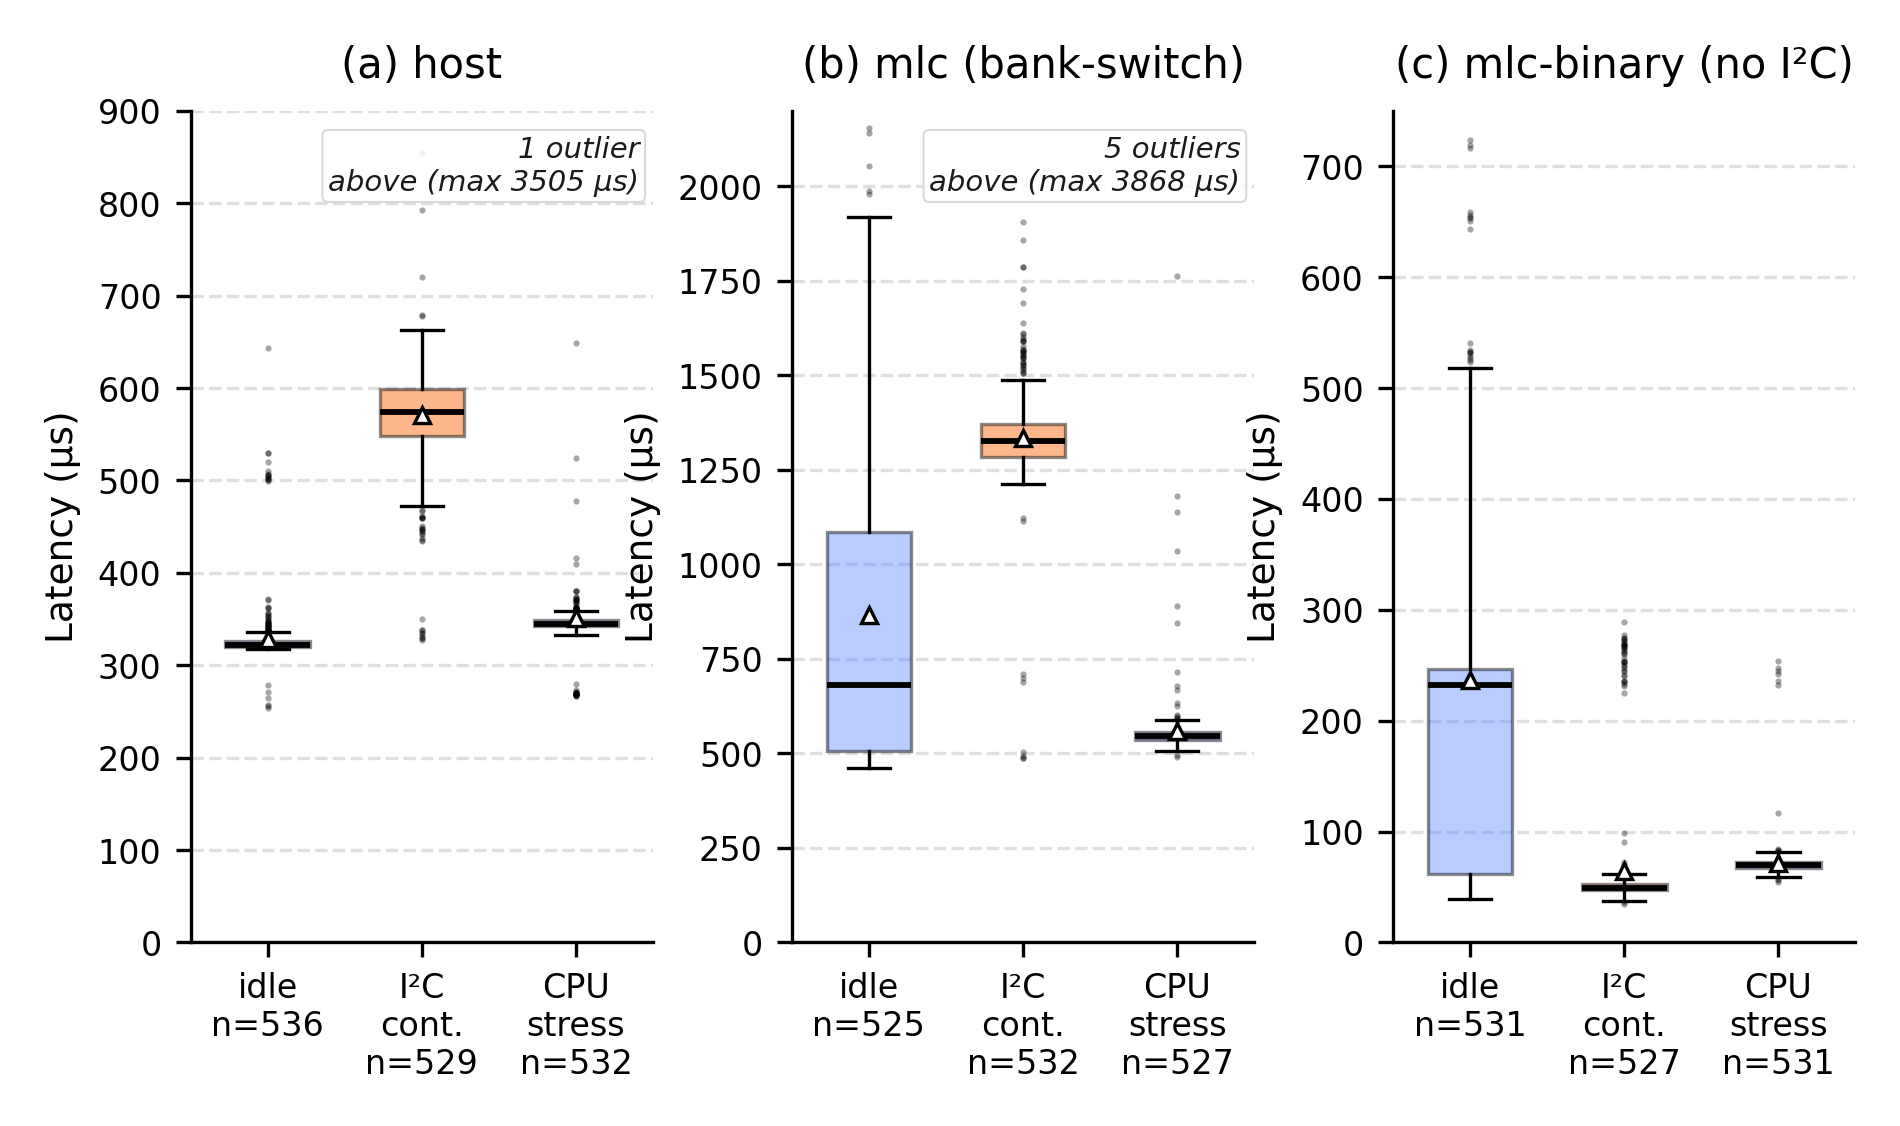
\includegraphics[width=\columnwidth]{figure_1_latency_boxplot.png}
  \caption{Per-trial wire-level latency by pipeline and condition. The mlc-binary panel (zero I\textsuperscript{2}C transactions on the decision path) isolates the kernel/gpiod latency floor; note the per-panel $y$-axis scaling.}
  \label{fig:latency}
\end{figure}

\begin{table}[!t]
  \centering
  \caption{Wire-Level Latency per Pipeline $\times$ Condition ($\mu$s)}
  \label{tab:latency}
  \setlength{\tabcolsep}{4pt}
  \footnotesize
  \begin{tabular}{llrrr}
    \toprule
    Pipeline & Condition & $n$ & Median & IQR (p25--p75) \\
    \midrule
    host       & idle      & 536 & 321.7  & 319.7--326.4   \\
    host       & i2c-cont. & 529 & 574.5  & 547.8--599.0   \\
    host       & stress    & 532 & 345.0  & 342.0--349.0   \\
    mlc        & idle      & 525 & 681.5  & 505.4--1086.8  \\
    mlc        & i2c-cont. & 532 & 1325.4 & 1283.8--1371.5 \\
    mlc        & stress    & 527 & 546.1  & 535.8--557.0   \\
    mlc-binary & idle      & 531 & 231.9  & 61.8--246.2    \\
    mlc-binary & i2c-cont. & 527 & 49.4   & 46.9--53.2     \\
    mlc-binary & stress    & 531 & 70.2   & 66.9--73.0     \\
    \bottomrule
  \end{tabular}
\end{table}

\subsection{Confirmatory tests}

\textbf{H1' (host < MLC at idle): SUPPORTED.} Host idle median (321.7 $\mu$s) is 359 $\mu$s below MLC bank-switch idle (681.5 $\mu$s), a 2.1$\times$ host speedup. The Hodges-Lehmann shift is $\Delta$HL = $-$359.3 $\mu$s, 95\% bootstrap CI [$-$373.6, $-$352.5] (10,000 iterations); Mann-Whitney p = 1.87 $\times$ 10\textsuperscript{-170}, rejected at the Holm-Bonferroni threshold across the {H1', H2', H3', H6', H7'} family.

\textbf{H2' (host < MLC under I\textsuperscript{2}C contention): SUPPORTED.} With three concurrent i2c\_hammer processes on bus 7, host median rises to 574.5 $\mu$s and MLC to 1,325.4 $\mu$s; the shift grows to $\Delta$HL = $-$753.2 $\mu$s [$-$760.0, $-$746.7] (2.3$\times$ advantage), p = 2.33 $\times$ 10\textsuperscript{-170}.

\textbf{H3' (MLC degrades more than host): SUPPORTED.} The $\Delta$-of-$\Delta$ contrast is +391.1 $\mu$s [+372.8, +400.0], p = 1.00 $\times$ 10\textsuperscript{-4}. The MLC degrades by +611.7 $\mu$s (+90\%, idle$\rightarrow$contention) versus the host's +249.2 $\mu$s (+78\%): the MLC's three-transaction I\textsuperscript{2}C read protocol amplifies the contention penalty.

\textbf{H5' (CPU stress null for host latency): SUPPORTED.} Host median rises only from 321.7 $\mu$s (idle) to 345.0 $\mu$s (stress); a TOST against the pre-registered $\pm$30 $\mu$s margin gives +23.3 $\mu$s, 90\% CI [+22.7, +23.7] $\subset$ [$-$30, +30]. Equivalence is declared; a 208 Hz polling loop does not contend with stress-ng for CPU time.

\textbf{H6' (CPU stress positive for energy): SUPPORTED.} Mean VDD\_IN (INA3221 via tegrastats) rises from 5,206 mW (idle) to 8,626 mW (stress): +3,420 mW [+3,410, +3,429], exceeding the pre-registered +1,000 mW threshold threefold. The power axis distinguishes CPU stress unambiguously where the latency axis (H5') cannot.

\textbf{H7' (MLC stability degrades under contention): FALSIFIED, direction opposite.} The fraction of stimulus windows with exactly one D1 rising edge is 97.22\% (525/540) at idle versus 98.89\% (534/540) under contention, a +1.67 percentage-point \emph{increase} rather than the predicted decrease. Fisher's exact test in the pre-registered direction gives p = 0.9874 (two-sided p = 0.0755). H7' is formally falsified in pre-registration v7.10 \cite{ref4}. I\textsuperscript{2}C contention slows the MLC pipeline (H2', H3') but does not degrade the silicon's classifier reliability.

\subsection{Multimodal latency distributions}

\textbf{Fig. 1} reveals previously-unreported multimodal structure in both MLC pipelines. The mlc/idle distribution is bimodal (mean 866.6 $\mu$s exceeds median 681.5 $\mu$s, with p95 reaching 1,780.7 $\mu$s), and mlc-binary/idle shows three modes near 60, 240, and 470 $\mu$s. Under contention and stress both collapse to tighter distributions, consistent with idle-state variance reflecting the kernel/I\textsuperscript{2}C scheduler's full timing-edge variability when not load-pinned. We report this as exploratory; the mechanism requires kernel-level (ftrace) instrumentation beyond this study's scope.

\subsection{MLC intrinsic decision cadence}

Inter-trial D0 (INT1) gaps (n = 3,086) cluster sharply at integer multiples of T = 706.5 ms with empty inter-peak bins. T equals one-quarter of the MLC's 75-sample, 26 Hz window period (2.885 s / 4 = 0.721 s; empirical peak 0.7065 s). This quantization is intrinsic to the silicon (classification updates only on the MLC's internal 706.5 ms clock), and we find it undocumented in ST application notes \cite{ref2} or the LSM6DSOX datasheet.

\subsection{Exclusion rates}

No cell exceeded the pre-registered 10\% exclusion ceiling (highest: mlc/idle, 2.78\%). The dominant exclusion category (68 of 90 trials) was multiple D1 edges per window, attributable to the 706.5 ms cadence interacting with stimulus-window boundaries.


\section{Discussion}

\subsection{The I\textsuperscript{2}C read protocol dominates wire-level latency}

The headline finding, that host classification is 2.1--2.3$\times$ faster than the on-sensor MLC under every tested condition, is explained by \textbf{Fig. 1(c)}: the mlc-binary pipeline, which performs zero I\textsuperscript{2}C transactions on the decision path (toggling D1 unconditionally on every INT1 edge), reaches a median of 49.4 $\mu$s under contention. The mlc-minus-mlc-binary difference under identical conditions isolates the I\textsuperscript{2}C read overhead at roughly 1,276 $\mu$s under contention (1,325.4 $-$ 49.4) and 476 $\mu$s under stress. This cost is not the silicon's classification time; it is the bank-switch read protocol's three-transaction sequence (write FUNC\_CFG\_ACCESS, read MLC0\_SRC, write it back) competing for bus arbitration.

Two consequences follow. Any platform using the LSM6DSOX MLC over I\textsuperscript{2}C inherits this overhead by construction: the bank-switch protocol is neither optional nor bypassable on the standard read path. And the overhead scales with bus contention, not classifier complexity: a deeper decision tree would not change the per-decision I\textsuperscript{2}C cost, but a busier bus would. The host-MLC gap is overwhelmingly a bus-protocol artifact, not a classifier-architecture one.

\subsection{Implications for safety-critical edge ML}

A naive reading of "on-sensor inference is faster" would favor the MLC for low-latency safety-critical loops such as exoskeleton control \cite{ref3}. Our results invert that on the wire-level latency axis: the host reaches its decision 359 $\mu$s earlier at idle, 753 $\mu$s earlier under contention, and is equivalence-null against CPU stress (H5').

The control results sharpen the practical lesson: \textbf{"stress" is not a single thing.} CPU stress is significant on energy (H6', +3,420 mW) but null on host latency (H5') and on classifier reliability; I\textsuperscript{2}C bus contention is significant on latency (H2', H3') but null on classifier reliability (H7' falsified; the stable-trial rate is, if anything, slightly higher under contention). A specification that bundles CPU stress and bus contention into one "stress margin" over-provisions one axis while under-provisioning the other: a shared I\textsuperscript{2}C bus demands a contention-aware latency budget, while CPU saturation on a clean bus leaves host latency essentially unaffected.

\subsection{Multimodal distributions and intrinsic cadence}

Two secondary findings carry safety-critical weight. First, the MLC pipelines are multimodal at idle (Section~V.B): the mlc/idle p95 of 1,781 $\mu$s is 2.6$\times$ its median, a factor that vanishes under a unimodal-Gaussian assumption. For a "worst latency observed with probability 1 $-$ $\varepsilon$" specification, the upper mode, not the median, is the relevant quantity.

Second, the 706.5 ms decision cadence (Section~V.C) is the dominant contributor to \emph{stimulus-to-decision} latency at the system level. Because the MLC fires only on its internal clock boundary, an unsynchronized real-world stimulus waits a uniformly-distributed 0--706.5 ms (mean 353 ms) before the silicon can respond. This is invisible on the D0-to-D1 wire-level axis we measured but is a structural floor; the 1--2 ms wire-level differences this paper characterizes are second-order against it.

\subsection{Limitations}

Results are specific to one platform, sensor IC family, bus protocol (I\textsuperscript{2}C, not SPI), ODR, and MLC configuration; the structural findings should transfer to similar ARM-edge + ST-MEMS combinations but require confirmation, and SPI access in particular could reduce the per-transaction overhead that drives our result. A pre-registered RT-scheduling (chrt+taskset) ablation was specified but not activated; pilot data suggesting it could roughly halve MLC contention latency makes it the most concrete next step.


\section{Conclusion}

We measured wire-level stimulus-to-decision latency for three pipelines on a Jetson Orin Nano + LSM6DSOX edge platform. Against the intuition that on-sensor inference is faster, the host pipeline achieves 2.1$\times$ lower median latency at idle and 2.3$\times$ lower under I\textsuperscript{2}C contention; the mlc-binary variant isolates the bank-switch read protocol's ~1,276 $\mu$s contention cost. The three-transaction I\textsuperscript{2}C read, not the silicon's classification, dominates. The control results show the safety-critical axis is which resource is contended: CPU stress registers on energy but not latency, I\textsuperscript{2}C contention the reverse. We document a 706.5 ms intrinsic MLC cadence imposing a 0--706.5 ms stimulus-to-decision wait. Code, data, and pre-registration: github.com/akulswami/sensor-mlc-latency.


% ---------------- Figures ----------------

% ---------------- Table ----------------

% ---------------- References ----------------
\begin{thebibliography}{11}

\bibitem{ref1} STMicroelectronics, ``LSM6DSOX: 6-axis IMU with machine learning core,'' Datasheet DS12140, 2024. [Online]. Available: https://www.st.com/resource/en/datasheet/lsm6dsox.pdf

\bibitem{ref2} STMicroelectronics, ``LSM6DSOX: Machine Learning Core,'' Application Note AN5259, 2023. [Online]. Available: https://www.st.com/resource/en/application\_note/an5259-lsm6dsox-machine-learning-core-stmicroelectronics.pdf

\bibitem{ref3} M.~Razmi and I.~Shojaei, ``Event-driven on-sensor locomotion mode recognition using a shank-mounted IMU with embedded machine learning for exoskeleton control,'' arXiv:2602.21418, Feb.\ 2026.

\bibitem{ref4} A.~Swami, ``Pre-registration chain for the sensor-mlc-latency study,'' Zenodo, externally-timestamped multi-amendment DOI chain (v6.1--v7.10), 2026. doi:10.5281/zenodo.20420866 (v7.10).


\bibitem{ref5} H.~B.~Mann and D.~R.~Whitney, ``On a test of whether one of two random variables is stochastically larger than the other,'' \emph{Ann. Math. Statist.}, vol.~18, no.~1, pp.~50--60, 1947.

\bibitem{ref6} J.~L.~Hodges and E.~L.~Lehmann, ``Estimates of location based on rank tests,'' \emph{Ann. Math. Statist.}, vol.~34, no.~2, pp.~598--611, 1963.

\bibitem{ref7} B.~Efron, ``Bootstrap methods: Another look at the jackknife,'' \emph{Ann. Statist.}, vol.~7, no.~1, pp.~1--26, 1979.

\bibitem{ref8} D.~J.~Schuirmann, ``A comparison of the two one-sided tests procedure and the power approach for assessing the equivalence of average bioavailability,'' \emph{J. Pharmacokinet. Biopharm.}, vol.~15, no.~6, pp.~657--680, 1987.


\bibitem{ref9} S.~Holm, ``A simple sequentially rejective multiple test procedure,'' \emph{Scand. J. Statist.}, vol.~6, no.~2, pp.~65--70, 1979.

\end{thebibliography}

\end{document}
